\documentclass[conference]{IEEEtran}
\IEEEoverridecommandlockouts
% The preceding line is only needed to identify funding in the first footnote. If that is unneeded, please comment it out.
\usepackage{cite}
\usepackage{amsmath,amssymb,amsfonts}
\usepackage{algorithmic}
\usepackage{graphicx}
\usepackage{textcomp}
\usepackage{xcolor}
\usepackage[ruled,vlined]{algorithm2e}
\def\BibTeX{{\rm B\kern-.05em{\sc i\kern-.025em b}\kern-.08em
		T\kern-.1667em\lower.7ex\hbox{E}\kern-.125emX}}
\begin{document}
	
	\title{Moving 3D Pose Estimation with ESP32 Wi-Fi \\
		{\footnotesize \textsuperscript{}}
		\thanks{}
	}
	
	\author{\IEEEauthorblockN{1\textsuperscript{st} Ratthamontree Burimas}
		\IEEEauthorblockA	{\textit{School of Information, Computer and}\\ \textit{Communication Technology} \\
			\textit{Sirindhorn International Institute of Technology}\\
			Pathum Thani, Thailand \\
			bank23232525@gmail.com}
		\and
		\IEEEauthorblockN{2\textsuperscript{nd} Teerayut Horanont}
		\IEEEauthorblockA
		{\textit{School of Information, Computer and}\\ \textit{Communication Technology} \\
			\textit{Sirindhorn International Institute of Technology}\\
			Pathum Thani, Thailand \\
			teerayut@siit.tu.ac.th}
	}
	
	
	
	
	
	
	\maketitle
	
	
	
	
	\begin{abstract}

		
	\end{abstract}
	
	\begin{IEEEkeywords}
		Channel State Information
	\end{IEEEkeywords}
	
	\section{Introduction}
		 Wifi is a common medium in many kinds of field nowadays. Normally, It is used for establishing a wireless network to connect to the internet. But there are still many more functions Wifi is good at. Wifi can also be applied in fields beside connecting to the internet according to its stability being upgraded continuously. Decent Wifi connectivity can extract more data other than the data to be transmitted like concentration, speed, obstacle between the transmission. Those can be composed to be many useful data on their own like localization, activity prediction and  etc.
		 
		 Camera is a very good tool for monitoring things and is being used as a very effective data collector for mapping to the ground truth to create many popular machine-learning-based usable model like pose estimation, text segmentation, object detection and many  more. However, camera are unavoidably judged as a serious privacy infringement since the data obtained like a photo or video are too clear and possess too much information that might be used in a bad way.
		 
		 There are many works tried to extract those extractable features like camera does from Wifi. But, they are mostly working with very specific tools and Network Interface Card (NIC) connected to a labtop running Linux that is currently one of the ways allowing to obtain fine-grain Channel State Information (CSI), the descriptive data of the  Wifi propagating in that environment. Those limitation significantly decrease steamline of implementation. It is hard for public demonstration and intregation with many updated tools in operating system like Windows or OSX.
		
		Actually, there are other existing ways for obtaining the CSI. One is from a ubiquitously used microprcessor ESP32. which is still not much be explored in exploiting Wifi field. It is simple to implement and can be easily integrated with others tools in many platforms due to its massively produced external tools. This paper proposes a machine-learning-based model to create a mapping rule from Wifi CSI to 3D moving human pose estimation by using ESP32.
	
	
	\section{Background}
	
	\subsection{Pose Estimation}
	
	There many machine-learning-based human body pose detection tools had been proposed and available online. Those can de found both 2D and 3D. In our paper, we chose a light weight 3D pose detection as an annotation due to its simplicity and the hypothesis that 3D should suit the most in our work. The project can be found at [github-lw3d] and is based on [paper-Lightweight OpenPose] and [paper- Single-Shot Multi-Person 3D Pose Estimation From Monocular RGB]. Its job is to simply create 3D human pose annotation from an image. Then, feed to our works training process as an annoation.
	
	
	\subsection{Wifi}\label{wifi}
	
	Wifi is a well-known connectivity with no wire needed (wireless). It has been used as a medium for connecting to the internet for over 10 years. However, the Wifi is the name covering IEEE 802.11 n/g/ac protocols. It mostly deliver data through 2.4/5GHz frequency with multiple channels. The bandwidth in each channel is 22MHz. the data are to be transmitted  pararelly with multiplexing technique named orthogonal frequency division multiplexing (OFDM). Each carrier may propagate to a reciever with encountering many obstacles. The effect of that situation is the Doppler Effect.
	So, Channel State Information (CSI) is represented as physical layer indicator that can be used to investigate how each channel propagate to the reciever or back to the transmitter.
	
	If a sender sends data to a reciever through Wifi, the data will be surely not transmitted without any loss.
	


	\subsection{CSI data}\label{CSI}
	As mentioned in \ref{wifi} that data propagating to the reciever while touching surrounding environment, the CSI is a variation of the data. The CSI can  be found at both sender and reciever since reciever may transmit data back.In this paper, We consider to mainly use CSI at the transmiter. Let the sender use the modulation method of 16-quadrature amplitude modulation (16-QAM) which one carrier can carry 4 bits. When the sender needs to send a '1111', the modulation returns $x=1+1i$ then, transmit to the reciever. At the reciever, let the obtained data is $y=0.8+0.9i$. So, the CSI can be computed by the variation $h=y/x=0.2+3.4i$.
	Human body is literally water which reflect radio wave like Wifi. [] and [] have proven that human body can affect the CSI.
	
	\subsubsection{ESP32}\label{ESP32}
	ESP32 is a popular single-board computer (SBC). With its affordable price and many available additional tools, ESP32 is commonly used in Internet of Things field. Moreover, it can be applied in research field. Quantitative CSI can be obtained from Wifi in ESP according to [Wi-ESP]. The number of available subcarriers in ESP32 is 64.
	
	According to the detail about Wifi mentioned in \ref{wifi}, the Wifi in ESP32 has some limitation. It supports only 2.4GHz frequency and can be set only one channel over a connection. The bandwidth of each channel is 22MHz which each frequency in the band is represented in 64 subcarriers 
	The CSI can be both obtain from Access point (AP) and station (STA) as shown in Fig.~\ref{fig:ESP32CSI01}.
	The frequency of each channel is as 802.11 standard.
	
	
	
	\begin{figure}[htbp]
		
		\centerline{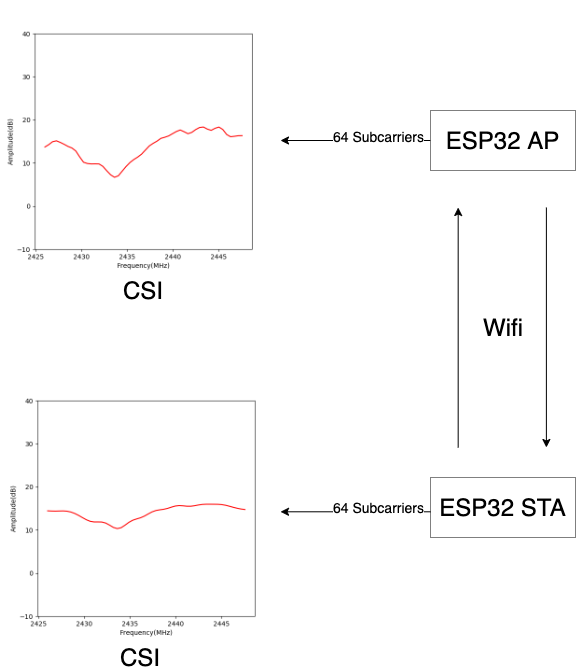
\includegraphics[width=70mm,scale=0.5]{ESP32CSI01.png}}
		\caption{CSI from ESP32s with channel 6.}
		\label{fig:ESP32CSI01}
	\end{figure}
	
	\iffalse
	\subsubsection{Faraday cage}
	Faraday cage is invented by Michael Faraday in 1836. It is an enclosure to block electromagnetic fields. It is made of conducting material which can affect any radio frequency (e.g. Wifi) to be unable to pass through.
	\fi
	\section{Proposed Method}
	
	\subsection{Concept}\label{AA}
	
	Other famous proposed works like [] [] and [] focus on line-of-sight (LOS) in between AP and STA while our work uses 2 directional Wifi antennae and focus on reflection from human body as shown in Fig.~\ref{fig:ESP32CSI02} on the left.
	
	The reason we name ``Moving Pose Detection" instead of ``Pose Detection" is that CSI is not only affected by human body but mainly by overall environment. This means that 2 corresponding human poses can result obviously different CSIs if the environment around are not exactly the same as shown in Fig.~\ref{fig:ESP32CSI02}.
	
	So, the detection of human standing still in every environment is nearly impossible since the CSI of that situation may be found exactly matched to a CSI of the environment that a big bottle of water placed in front of ESP32.
	In short, if it does not move, we do not if it is human.
	
	Meanwhile, the moving pose is totally different because we focus on its change instead. In different environment , the CSIs are  different. But, the corresponding moving pose may affect to the same changing pattern of CSI. This hypothesis is investigated in the upcoming parts.
	
	\begin{figure}[htbp]
		
		\centerline{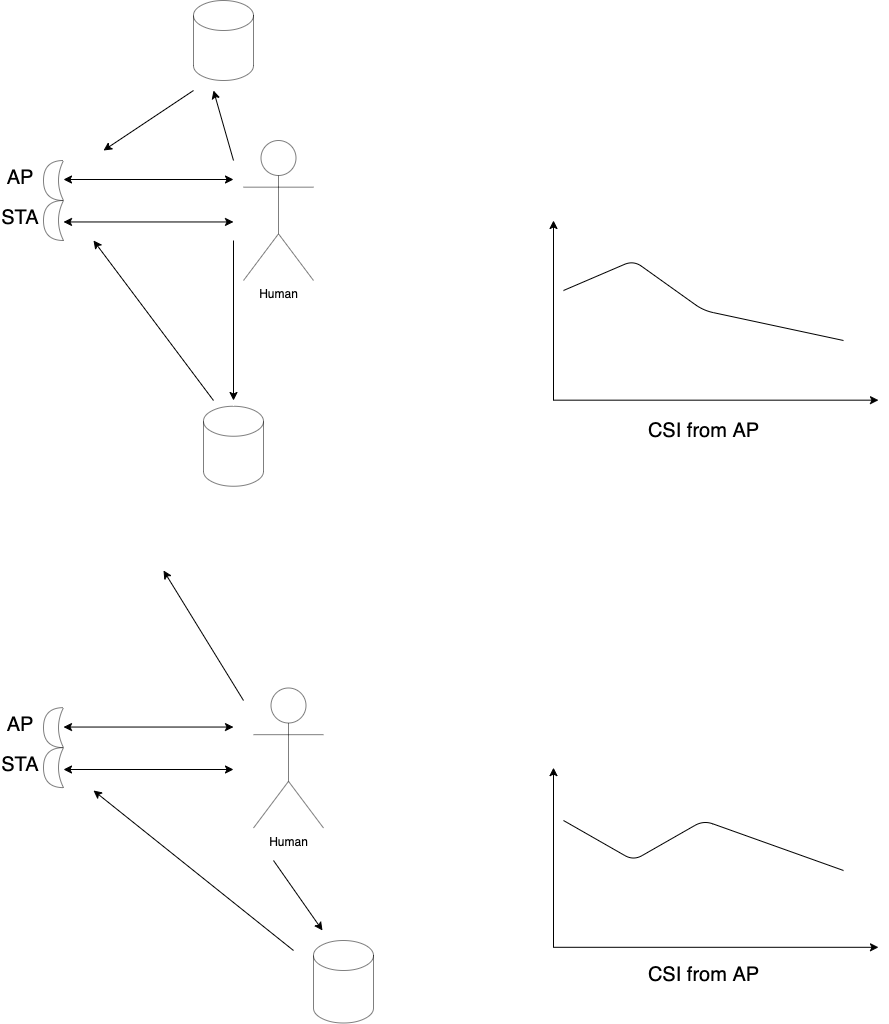
\includegraphics[width=70mm,scale=0.5]{ESP32CSI02.png}}
		\caption{2 different CSIs resulted from corresponding human poses.}
		\label{fig:ESP32CSI02}
	\end{figure}
	
	\iffalse
	 \subsection{CSI Clipping}
	 
	 The typically obtained CSI is a measurement of the traffic in an area where the signal propagate. The area may be considerably too big since the CSI can be affected by any unstable environment that is out of our focus e.g. we are focusing on a human standing still 3 meters away from the device but, the CSI is significantly fluctuated by a dog jumping 10 meters away from the device. Those uncontrollable factors are obvious not included in the annotation. So, it causes bad result in both training and testing processes. 
	 
	 To solve this, we use IFFT to turn the CSI into Power Delay Profile (PDP). The PDP is time-to-signal-power value where we can distinguish how strong signal power arrive at a certain time and we know that the signal normally travel at speed of light. Then, we filter out the PDP in the range that is surely arrive from a time range that is not in our focus e.g. we are focusing in an area of 7.5 meters then, we ignore the signal that arrive at the time after $(7.5/speed-of-light)= 2.25$ nanoseconds. Finally, we use FFT to turn the clipped PDP back into the CSI and use that CSI for further processing.
	 
	  Fig.~\ref{fig:CSIClipping01} top-left shows the originally obtained CSI. Then, it was turn into the PDP by IFFT (Fig.~\ref{fig:CSIClipping01} top-right). And, let time domain more than $10$ is considered out of focus. So, the PDP after time $10$ are forced to be $0$ in Fig.~\ref{fig:CSIClipping01} bottom-left. The clipped CSI where affected only from objects within the distance we focus is resulted back by FFT from the clipped PDP in Fig.~\ref{fig:CSIClipping01} bottom-right.
	 
	 \begin{figure}[htbp]

	 	\centerline{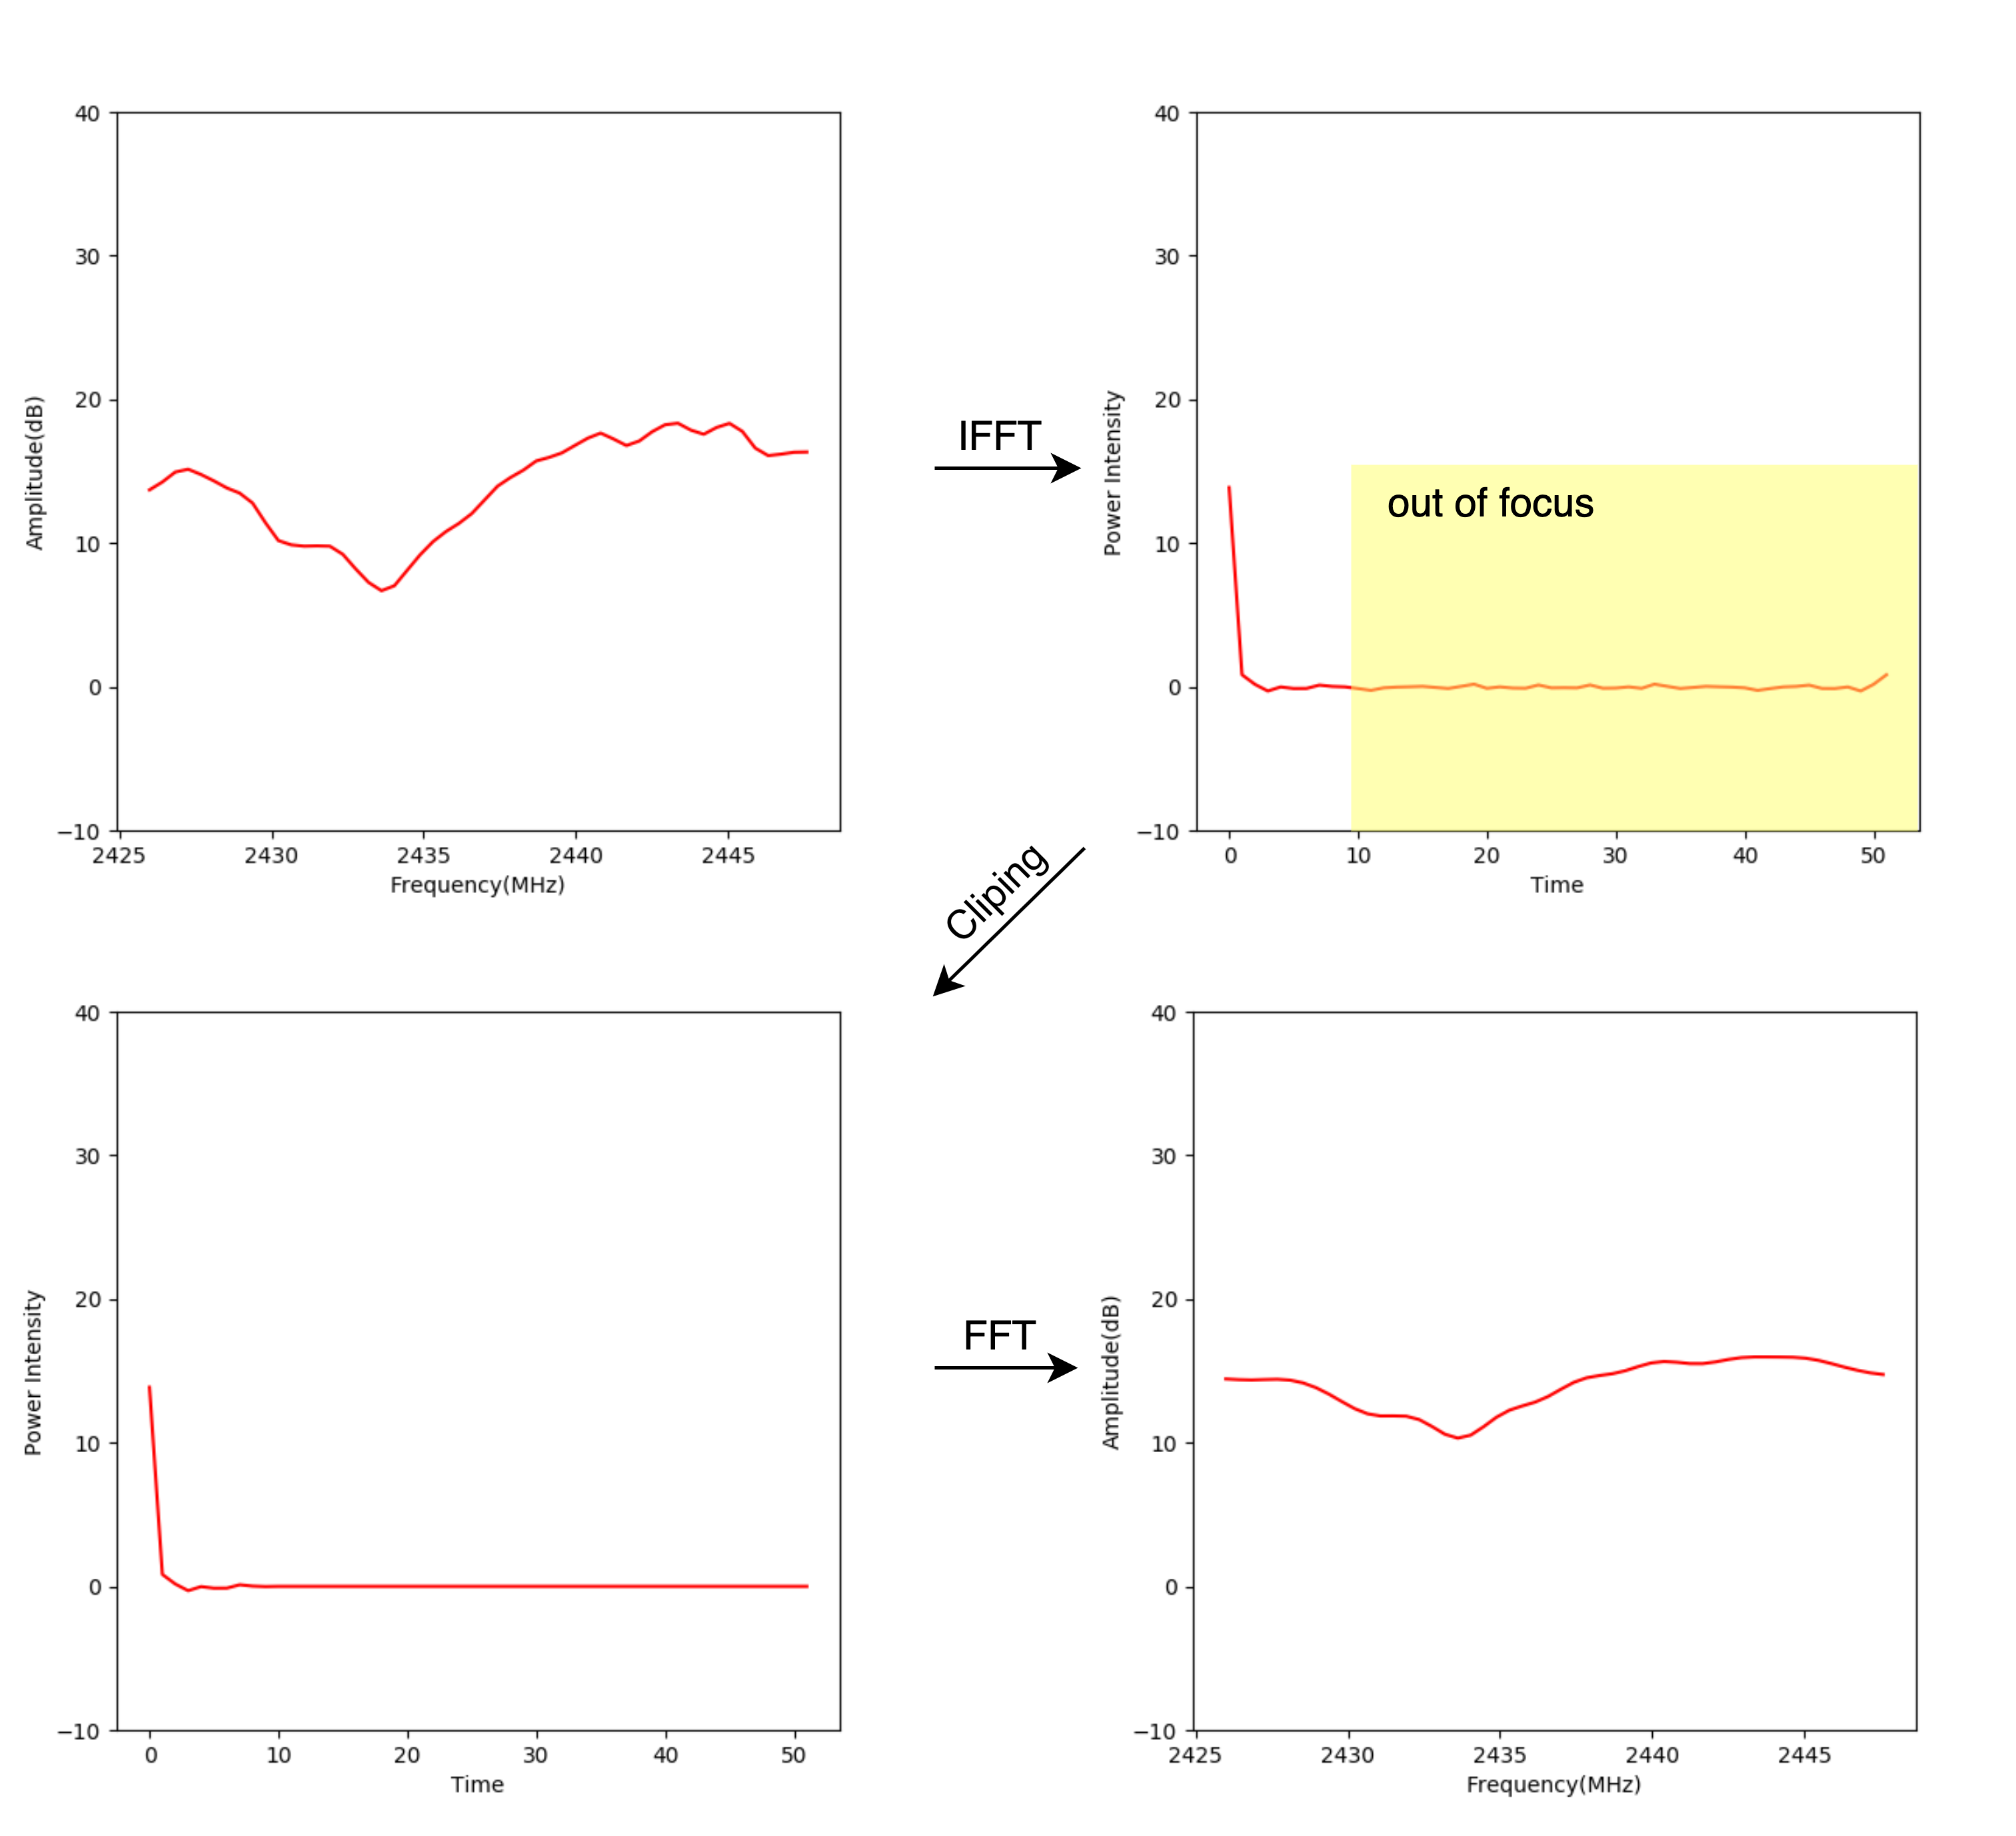
\includegraphics[width=70mm,scale=0.5]{CSIClipping01.png}}
	 	\caption{CSI clipping.}
	 	\label{fig:CSIClipping01}
	 \end{figure}
	 
	 \subsection{CSI Splicing}
	
	As mentioned in the above section, we can simply cliping the CSI to maintain only the part within the range we focus by using the PDP. But, the normal resolution of PDP is usually not that high. In short, the PDP resolution $\Delta\tau$ is depended on the CSI bandwidth. In 802.11n, the bandwidth is 22 MHz for one Wi-Fi channel. And, $\Delta\tau = 1/B$, where $B$ is the bandwidth.
	So, the PDP resolution $\Delta\tau$ in a normal CSI data is $1/(22*10^6)= 45.5$ nanoseconds (in Fig.~\ref{fig:CSISplicing01} top) which can separate the distance of
	$(45.5*speed-of-light)= 13.6$ meters. The 13-meter-gap is significantly not practical in our work.
	
	To enhance the PDP resolution, a straightforward idea is to expand the CSI bandwidth. There is a method called CSI Splicing proposed by []. This leads to the collections of CSI from many channels and merge with some error filtering to create a single CSI with the bandwidth of $\le$ 160MHz. 
	
	
	The fully spliced CSI with max bandwidth can result the PDP with resolution $\Delta\tau=1/(160*10^6)=6.25$  nanoseconds (in Fig.~\ref{fig:CSISplicing01} bottom) which allow us to separate the distance of
	$(6.25*speed-of-light)= 1.87$ meters.
	
		The example of merging CSI from Wi-Fi channel 1, 4, 6, 8 and 11 into single CSI with bandwidth 73 MHz is show in Fig.~\ref{fig:CSISplicing02}.
	
	\begin{figure}[htbp]
		
		\centerline{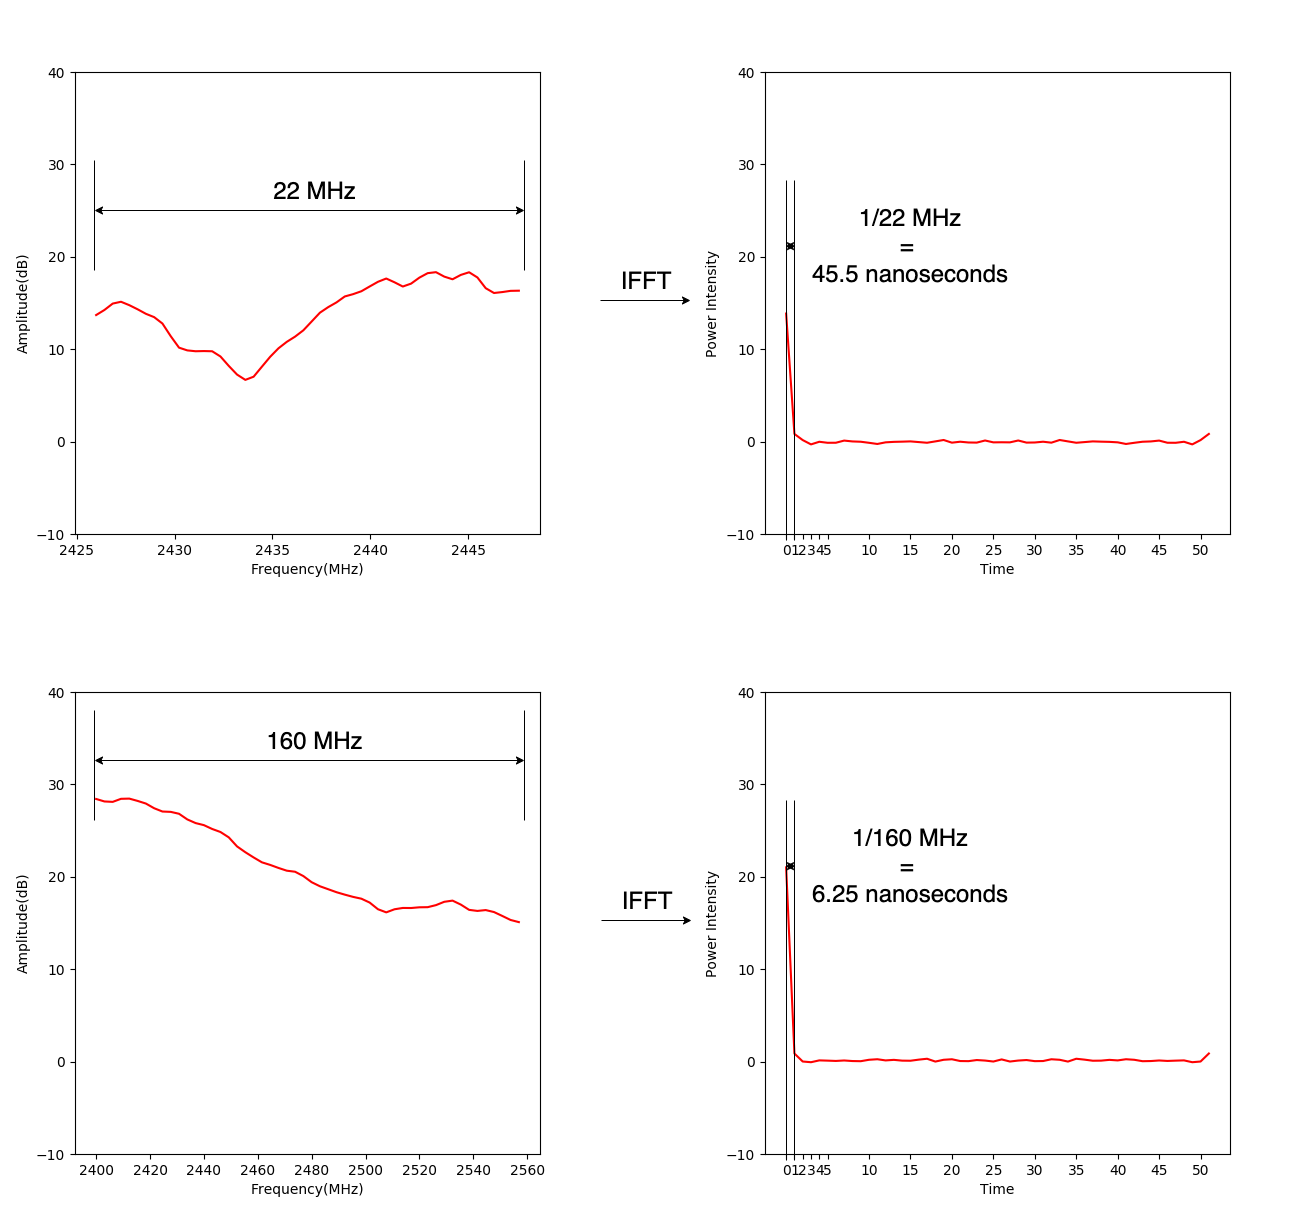
\includegraphics[width=70mm,scale=0.5]{CSISplicing01.png}}
		\caption{PDP resolution depending on CSI bandwidth.}
		\label{fig:CSISplicing01}
	\end{figure}

\begin{figure}[htbp]
	
	\centerline{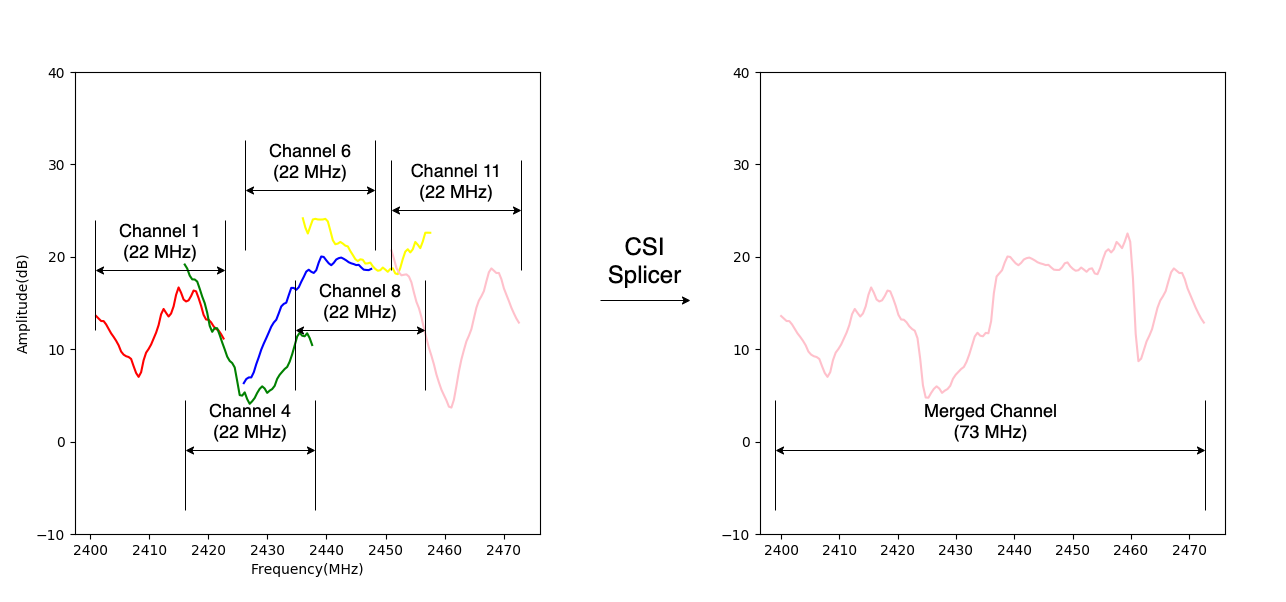
\includegraphics[width=70mm,scale=0.5]{CSISplicing03.png}}
	\caption{CSI splicing.}
	\label{fig:CSISplicing02}
\end{figure}
	
		\fi
	


	\subsection{Pre-processing}\label{Processing}
	
		A summation of all steps in our method is shown in Fig.~\ref{fig:STEP02}. 
	
	
	\begin{figure}[htbp]
		\centerline{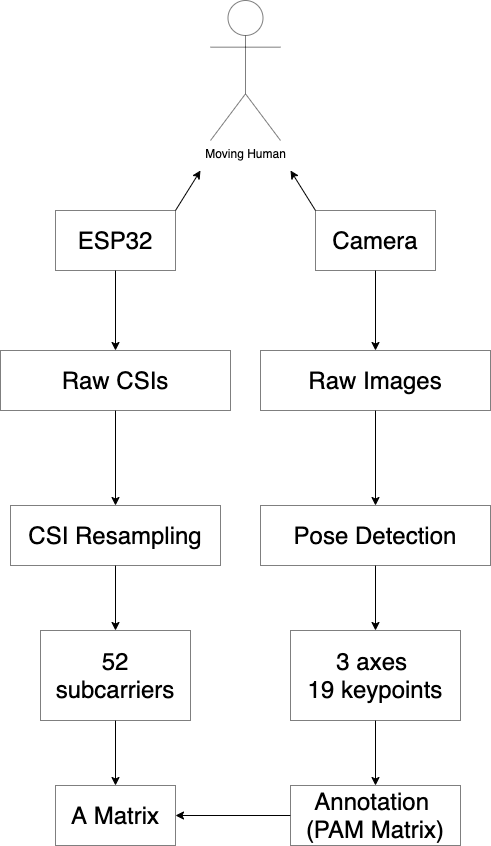
\includegraphics[width=70mm,scale=0.5]{STEP03.png}}
		\caption{A summation of all steps.}
		\label{fig:STEP02}
	\end{figure}
	
	\subsubsection{CSI Preparation}
	
		
	As mentioned in \ref{ESP32}, There are 64 subcarriers in CSI data from ESP32 but there are only 52 those are usable the rest are null. So, we can construst a tensor of $1 \times 52$ to represent each CSI. We are to map 3D human pose annotation from a camera to CSI from the ESP32. The sampling rate of the camera are set to 30Hz. So, we have 30 human pose annotations for one second. For the ESP32, the sampling rate is unpredictable and not constant but it is running around 120Hz. So we do a process called ``Resampling" to obtain CSI at rate 30Hz in order to map to each human pose annotation.
	
	An example of CSI Resampling is shown in Fig.~\ref{fig:CSIResampling01}. The top graph shows that the the original CSI is logged unstably. The bottom one is to pick a timestamp at rate 30Hz and calculated each with the closet data from the original with a simple mathamatical weight equation as in Eq.~\ref{eq:CSIResampling01} in order to predict CSI at timestamp corresponding to each human pose annotation.
	
	\begin{equation}
		\begin{aligned}
		& CSI_{now} = CSI_{before} \\ 
		& + \left(  \frac{ts_{now}-ts_{before}}{ts_{after}-ts_{before}}  \times (CSI_{after}-CSI_{before})   \right)
		\label{eq:CSIResampling01}
		\end{aligned}
	\end{equation},
		where ....
	
	\begin{figure}[htbp]
		\centerline{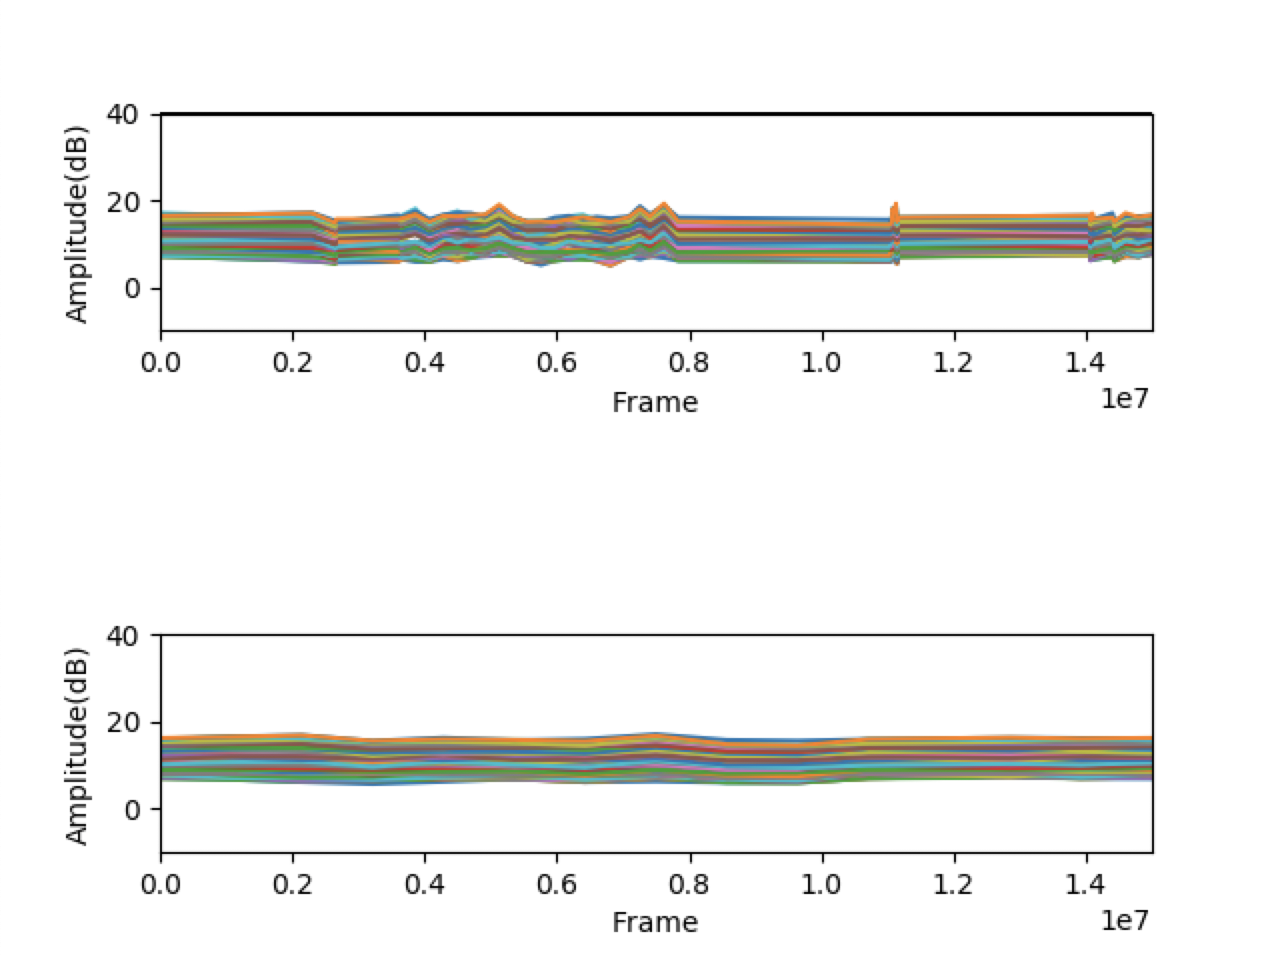
\includegraphics[width=70mm,scale=0.5]{CSIResampling01.png}}
		\caption{An example of CSI resampling.}
		\label{fig:CSIResampling01}
	\end{figure}
	
	Now we can map one CSI samples to one 3D human pose annotations from one images with the corresponding timestamp.
	

	\subsubsection{Human-Pose Preparation}
	
	A matrix of $19 \times 3$ are used as an annotation where $19$ is for keypoints in human body and $3$ is for 3 axes coordination as shown in Fig.~\ref{} But, the annotation can still possess too much independency. Some alignment of keypoints may lead to some impossible pose e.g. body keypoint found very far from neck keypoint or right shoulder keypoint attached to left knee keypoint. We assume those poses are quite not possible for normal human pose. To preserve those constraint, we form pose adjacent matrix (PAM) from an original $19\times3$ matrix. the PAM is applied for all x, y and z axes. Each are to be form their $19\times19$ matrix by the following equations.
	
	\begin{equation}
	x_{i,j}' = \begin{cases}
	x_i-x_j &\text{$i\neq j$}\\
	x_i &\text{$i=j$}\\
	\end{cases}
	\label{eq:xPAM}
	\end{equation},
	\begin{equation}
	y_{i,j}' = \begin{cases}
	y_i-y_j &\text{$i\neq j$}\\
	y_i &\text{$i=j$}\\
	\end{cases}
	\label{eq:yPAM}
	\end{equation}
	and
	\begin{equation}
	z_{i,j}' = \begin{cases}
	z_i-x_j &\text{$i\neq j$}\\
	z_i &\text{$i=j$}\\
	\end{cases}
	\label{eq:zPAM}
	\end{equation}.
	
	The PAM is finally a $3\times19\times19$ matrix created from 3 matrices of $x'$,$y'$ and $z'$ stacked.
	Apparently, one PAM represent one human pose.
	

	
	Conclusively, we are making a model by mapping a tensor of $1\times52$ from CSI to each tensor of $ 19 \times 3 \times 3 $ PAM from moving human pose annotation with the corresponding timestamp as shown in Fig.~\ref{fig:STEP01}. 
	
	\begin{figure}[htbp]
		\centerline{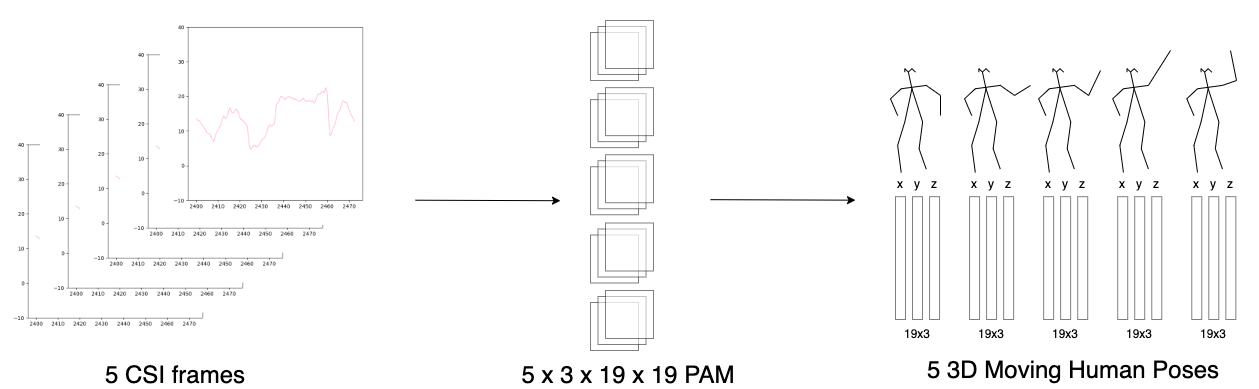
\includegraphics[width=70mm,scale=0.5]{STEP01.png}}
		\caption{A mapping rule from 5 CSI frames to 5 human poses.}
		\label{fig:STEP01}
	\end{figure}
	
	
	
	\subsection{Processing}

	
	\subsubsection{Data Alignment}
	Let $D$ be a set synchronized images and CSI data package. Each pair has corresponding timestamp.
	
	\begin{equation}
	D =  {(I_t, C_t), t \in [1, n]}
	\label{eq:Dataset}
	\end{equation}, where  $n$ is a number of pairs, $I_t$ is for PAM annotation as the ground truth, $C_t$ is for CSI data from ESP32, $t$ is the timestamp when those 2 were collected and $n$ is the number of data.
	
	$\sigma$ frames and CSIs are fed to the model concurrently. 
	
	\subsubsection{Form Network Layer}
	
	feed each $\pi$ of $D$
	
	
	LSTM
	\iffalse
	  We use ((Teacher and Student as [] and [])). Let the lightweight 3D human pose [] be a teacher network and our works (ESP32 pose sense) be a student network. The teacher and student network are termed as $T(·)$ and $S(·)$, respectively. 
	  
	  Iteratively, $T(·)$ takes $I_t$ then, returns a single 3D human pose as a matrix of $19 \times 3$ . And, we convert the obtained matrix to PAM with Eq.~\ref{eq:xPAM}, Eq.~\ref{eq:yPAM} and Eq.~\ref{eq:zPAM}. In short, $T(·)$ is formulized  as $T(I_t) \rightarrow PAM_t$. Recall that main purpose of $T(I_t)$ is to teach $S(·)$.
	 
	 Simultaneously, $S(·)$ takes $C_t$  then, returns the  prediction of PAM matrix.
	 The $S(·)$ is to be supervised by $T(·)$ until $S(·)$ can predict PAM close to the one at the $T(·)$. The process of transfroming from $C_t$ to $PAM_t$ is shown in Fiq.~\ref{}. There are 3 modules to achieve the transformation those are the encoder, feature extractor and the decoder.
	 
	 
	 	\paragraph{Encoder}
	 	The encoder takes CSI series ($5\times64$ matrix) as an input and outputs a tensor ($320\times148\times148$  matrix). The main purpose of the process is to upsample $C_t$ since ResNet[] is the convolutional network that is used in our work and it requires higher dimension of input. A single $C_t$ is 
	 	$5\times64$ matrix. We need to map it to a single RGB image which is $3\times244\times244$ matrix, where 3 is for 3 channel of colors and 224s are the dimension of the image. [CSI-NET] uses 8 stacked transposed convolutional layers to upsample and [WiSPPN] uses one
	 	bilinear interpolation operation. In our work, we decide to use ..... to convert $C_t$ to $320\times148\times148$  matrix.
	 	
	 	
	 	
	 	
	 	\paragraph{Feature Extractor}
	 	The feature extractor is the main part of training how to extract 3D human pose feature from the upsampled $C_t$. CSI data does not obviously contain any spatial information. So, we need to use deep network to enhance the feature extractor so that it can extract spatial infomarion from the CSI. Resnets [] is responsible for this job..................... The feature extractor consists of 4 stacked blocks of ResNet [] as shown in Fig.~\ref{}. The parameter of each layer is shown in Table \ref{}. At the end, we obtained $300\times19\times19$  matrix as a feature output $F_t$.
	 	
	 	
	 	
	 	1st block : Take a tensor ($320\times148\times148$   matrix) as an input and outputs a tensor ($320\times148\times148$  matrix)
	 	
	 	2nd block : Take a tensor ($320\times148\times148$   matrix) as an input and outputs a tensor ($150\times74\times74$  matrix)
	 	
	 	3rd block : Take a tensor ($150\times74\times74$   matrix) as an input and outputs a tensor ($300\times37\times37$  matrix)
	 	
	 	4th block : Take a tensor ($300\times37\times37$   matrix) as an input and outputs a tensor ($300\times19\times19$  matrix)
	 	
	 	\paragraph{Decoder}
	 	
	 	the decoder takes a $F_t$ ($300\times19\times19$  matrix) as an input and outputs the prediction of PAM ($3\times19\times19$ matrix). Its main job is to return the prediction of 3D human pose in a form of PAM where can be simply turned into 3D human pose. To do so,	 we stack two convolutional layers as shown in Fig.~\ref{}.(( Conv1 is mainly to release channel-wise information (from 300 to 36); and Conv2 is
	 	mainly to further reorganize spatial information of Ft with the 1 × 1 convolutional kernels.))
	 	
	 	
	 	To be concluded, these 4 modules are the step to turn CSI data series into predicted 3D human pose which is as $S(C_t) \rightarrow pPAM_t$. As this is teacher and student network, we believe that $pPAM_t$ is initially not correct and needed to be supervised by the $T(I_t) \rightarrow PAM_t$. Eventually, we obtain $S()$ that can predict 3D human pose effectively. The loss computation and the training of $S()$ are discussed further.

	
	\subsubsection{Pose Adjacent Matrix Similarity Loss}
	 
	 The $T()$ is to supervise the $S()$ with the PAM from images and Lightweight 3D human pose esitmation. L2 loss is applied for optimizing the $S()$.
	 \begin{equation}
	 \begin{aligned}
	 L = & \mid \mid pPAM^x \text{ - } PAM^x \mid \mid^2_2 + \\
	  & \mid \mid  pPAM^y \text{ - } PAM^y \mid \mid^2_2 + \\
	  & \mid \mid pPAM^z \text{ - } PAM^z \mid \mid^2_2
	 \label{eq:L2}
	 \end{aligned}
	 \end{equation}, where $\mid \mid  \mid \mid^2_2$ is an operator to compute L2 distance. $\text{pPAM}^x$, $\text{pPAM}^y$ and $\text{pPAM}^z$, from the $S()$, are the predictions  of PAM of 3D human pose on x-axis, y-axis and z-axis respectively. And, $\text{PAM}^x$, $\text{PAM}^y$ and $\text{PAM}^z$, from the $T()$, are the annotations of PAM of 3D human pose on x-axis, y-axis and z-axis respectively.
	 
	  
	 \subsection{Training Details and Pose Association}
	 
	 The environment of the implementation is python 3.7.9, scipy 1.6.0 and pytorch 1.7.1.
	 The network is trained for ... epochs with initial learning
	 rate of ...., batch size of ... and Adam optimizer. The learning rate decays by ... at the epoch of
	 5th, 10th and 15th.

	When the $S()$ is smart enough, we let it take 5 CSI data series as input and output pPAM on its own. Obviously, we can look at only diagonal values of the pPAM and plot 3D human pose on 3D canvas.
	
	
	\begin{equation}
	 \begin{aligned}
	 x_k^*,y_k^*,z_k^* = & \text{ for ($k = 1 \rightarrow 19$ ):} \\
	  & (pPAM_{1,k,k},pPAM_{2,k,k},pPAM_{3,k,k})
	 \end{aligned}
	\end{equation}
	\fi
	
	\section{Evaluation}
	
	\subsection{Data Collection}
	dance in ma room
	((
	We collected data under an approval of Carnegie Mellon University IRB 4
	. We recruited 8 volunteers,
	and asked them to do casual daily actions in two rooms of the campus, one laboratory room and one
	class room. Floor plans and data collection positions are illustrated in Fig. 8. During the actions, we
	run the system in Fig. 3 to record CSI samples and videos, simultaneously. For each volunteer, data
	of his first 80% recording is used to train the networks, and data of the last 20% recording is used to
	test the networks. The data size of training and testing are 79496 and 19931, respectively))
	
	
	\subsection{Experimental Result}
	Percentage of Correct Keypoint (PCK) is widely used to evaluate the performance of human pose estimation according to [].

	\begin{equation}
	\begin{aligned}
	PCK_i@a = \frac{1}{N} \sum_{i=1}^{N}
	I(
	\frac{\mid \mid  pd_i \text{ - } gt_i \mid \mid^2_2}{\sqrt{rh^2+lh^2}}  \le a ),
	\label{eq:PCK}
	\end{aligned}
	\end{equation}
	
	
	where $I$(·) is a binary indicator that outputs 1 while true and 0 while false, 
	$N$ is the number of frames, $i$ is the index of keypoints that $i \in {1, 2, ..., 19}$. The $rh$ and
	$lh$ are for the positions of the right shoulder and the left hip from the ground truth, respectively.
	So, the ${\sqrt{rh^2+lh^2}}$ is  considered as the length of the upper limb from the ground truth, which is used to normalize the prediction error length
	$ \mid \mid pd_i \text{ - } gt_i \mid \mid _2^2$, and $pd_i$ and $gt_i$ are coordinates of prediction and ground-truth at the keypoint $i$ repectively.
	
	
	[Table.~\ref{table:PCK}] shows the estimation performance of 19 body keypoint in PCK@5, PCK@10, PCK@20,
	PCK@30, PCK@40, and PCK@50 of the frame length $15$, isActSDthreshold is $100$ and minCSIthreshold is $40$.
	
	
	
	
	
 Github$\footnote[1]{https://github.com/rtmtree/}$.

	

\begin{table*}[]
	\caption{Wifi2Pose Evaluation}
	\label{table:PCK}
	\begin{tabular}{|l|l|l|l|l|l|l|l|}
		\hline
		Order & Keypoint & PCK@5 & PCK@10 & PCK@20 & PCK@30 & PCK@40 & PCK@50 \\ \hline
		1     &          &       &        &        &        &        &        \\ \hline
		2     &          &       &        &        &        &        &        \\ \hline
		3     &          &       &        &        &        &        &        \\ \hline
		4     &          &       &        &        &        &        &        \\ \hline
		5     &          &       &        &        &        &        &        \\ \hline
		6     &          &       &        &        &        &        &        \\ \hline
		7     &          &       &        &        &        &        &        \\ \hline
		8     &          &       &        &        &        &        &        \\ \hline
		9     &          &       &        &        &        &        &        \\ \hline
		10    &          &       &        &        &        &        &        \\ \hline
		11    &          &       &        &        &        &        &        \\ \hline
		12    &          &       &        &        &        &        &        \\ \hline
		13    &          &       &        &        &        &        &        \\ \hline
		14    &          &       &        &        &        &        &        \\ \hline
		15    &          &       &        &        &        &        &        \\ \hline
		16    &          &       &        &        &        &        &        \\ \hline
		17    &          &       &        &        &        &        &        \\ \hline
		18    &          &       &        &        &        &        &        \\ \hline
		19    &          &       &        &        &        &        &        \\ \hline
	\end{tabular}
\end{table*}
	

	
	
	\section*{Conclusion and Future Development}

	This paper proposes 2 algorithms for 2 simplification types, Fixed-\# and Fixed-LSSED. Classically, to achievement the best satisfying result for both types, the time complexity of $O(2^{N-2})$ is needed, where $N$ is a number of trajectory point. By exploiting quantum mechanics from the QSMA, we can do the same job by consuming only the time complexity of $O(\frac{\pi}{2}\sqrt{\frac{2^{N-2}}{M}} \times c)$, where $M$ is a number of the finest solution and $c$ is an adjustable parameter.
	

	
	\section*{Acknowledgment}
	
	We thank Sirindhorn International Institute of Technology for providing technical environment and supportive information.
	
	
	
	
	\begin{thebibliography}{00}
		\bibitem{b0} Y. Chen, S. Wei, X. Gao, C. Wang, J. Wu and H. Guo, ``An Optimized Quantum Maximum or Minimum Searching Algorithm and its Circuits,'' arXiv:1908.07943 [quant-ph] 21 Aug 2019.
		\bibitem{b1} G. L. Long, ``Grover algorithm with zero theoretical failure rate,''	arXiv:quant-ph/0106071, 13 Jun 2001.
		\bibitem{b2} A. Ahuja and S. Kapoor, ``A Quantum Algorithm for finding the Maximum,''	arXiv:quant-ph/9911082, 18 Nov 1999.
		\bibitem{b3} C. Dürr and P. Høyer, ``A quantum algorithm for finding the minimum,''	arXiv:quant-ph/9911082, 18 Nov 1999.
		
		\bibitem{b4} M. Chen, M. Xu and P. Fränti, ``A Fast Multiresolution Polygonal
		Approximation Algorithm for GPS
		Trajectory Simplification,'' IEEE Transactions on image processing, col. 21, No. 5, May 2012.
		
		\bibitem{b5} D. Zhang, M. Ding, D. Yang, Y. Liu, J. Fan, H. T. Shen, ``Trajectory Simplification: An Experimental Study and Quality Analysis,'' Proceedings of the VLDB Endowment, vol. 11, No. 9, Rio de Janeiro, Brazil, August 2018.
		\bibitem{b6} N. Meratnia and R. A. de By, ``Spatiotemporal compression techniques for moving point objects,'' In EDBT, pages 765–782, 2004.
		
		
		
		
	\end{thebibliography}
	
\end{document}
